% Options for packages loaded elsewhere
\PassOptionsToPackage{unicode}{hyperref}
\PassOptionsToPackage{hyphens}{url}
%
\documentclass[
]{article}
\title{LPG v/s Firewood}
\author{}
\date{\vspace{-2.5em}}

\usepackage{amsmath,amssymb}
\usepackage{lmodern}
\usepackage{iftex}
\ifPDFTeX
  \usepackage[T1]{fontenc}
  \usepackage[utf8]{inputenc}
  \usepackage{textcomp} % provide euro and other symbols
\else % if luatex or xetex
  \usepackage{unicode-math}
  \defaultfontfeatures{Scale=MatchLowercase}
  \defaultfontfeatures[\rmfamily]{Ligatures=TeX,Scale=1}
\fi
% Use upquote if available, for straight quotes in verbatim environments
\IfFileExists{upquote.sty}{\usepackage{upquote}}{}
\IfFileExists{microtype.sty}{% use microtype if available
  \usepackage[]{microtype}
  \UseMicrotypeSet[protrusion]{basicmath} % disable protrusion for tt fonts
}{}
\makeatletter
\@ifundefined{KOMAClassName}{% if non-KOMA class
  \IfFileExists{parskip.sty}{%
    \usepackage{parskip}
  }{% else
    \setlength{\parindent}{0pt}
    \setlength{\parskip}{6pt plus 2pt minus 1pt}}
}{% if KOMA class
  \KOMAoptions{parskip=half}}
\makeatother
\usepackage{xcolor}
\IfFileExists{xurl.sty}{\usepackage{xurl}}{} % add URL line breaks if available
\IfFileExists{bookmark.sty}{\usepackage{bookmark}}{\usepackage{hyperref}}
\hypersetup{
  pdftitle={LPG v/s Firewood},
  hidelinks,
  pdfcreator={LaTeX via pandoc}}
\urlstyle{same} % disable monospaced font for URLs
\usepackage[margin=1in]{geometry}
\usepackage{graphicx}
\makeatletter
\def\maxwidth{\ifdim\Gin@nat@width>\linewidth\linewidth\else\Gin@nat@width\fi}
\def\maxheight{\ifdim\Gin@nat@height>\textheight\textheight\else\Gin@nat@height\fi}
\makeatother
% Scale images if necessary, so that they will not overflow the page
% margins by default, and it is still possible to overwrite the defaults
% using explicit options in \includegraphics[width, height, ...]{}
\setkeys{Gin}{width=\maxwidth,height=\maxheight,keepaspectratio}
% Set default figure placement to htbp
\makeatletter
\def\fps@figure{htbp}
\makeatother
\setlength{\emergencystretch}{3em} % prevent overfull lines
\providecommand{\tightlist}{%
  \setlength{\itemsep}{0pt}\setlength{\parskip}{0pt}}
\setcounter{secnumdepth}{-\maxdimen} % remove section numbering
\ifLuaTeX
  \usepackage{selnolig}  % disable illegal ligatures
\fi

\begin{document}
\maketitle

{
\setcounter{tocdepth}{2}
\tableofcontents
}
\newpage

\hypertarget{characteristics-of-the-sample}{%
\section{Characteristics of the
Sample}\label{characteristics-of-the-sample}}

The following graph shows that distribution of different demographic
variables in our sample of 2,160 from the combined dataset from both
surveys.

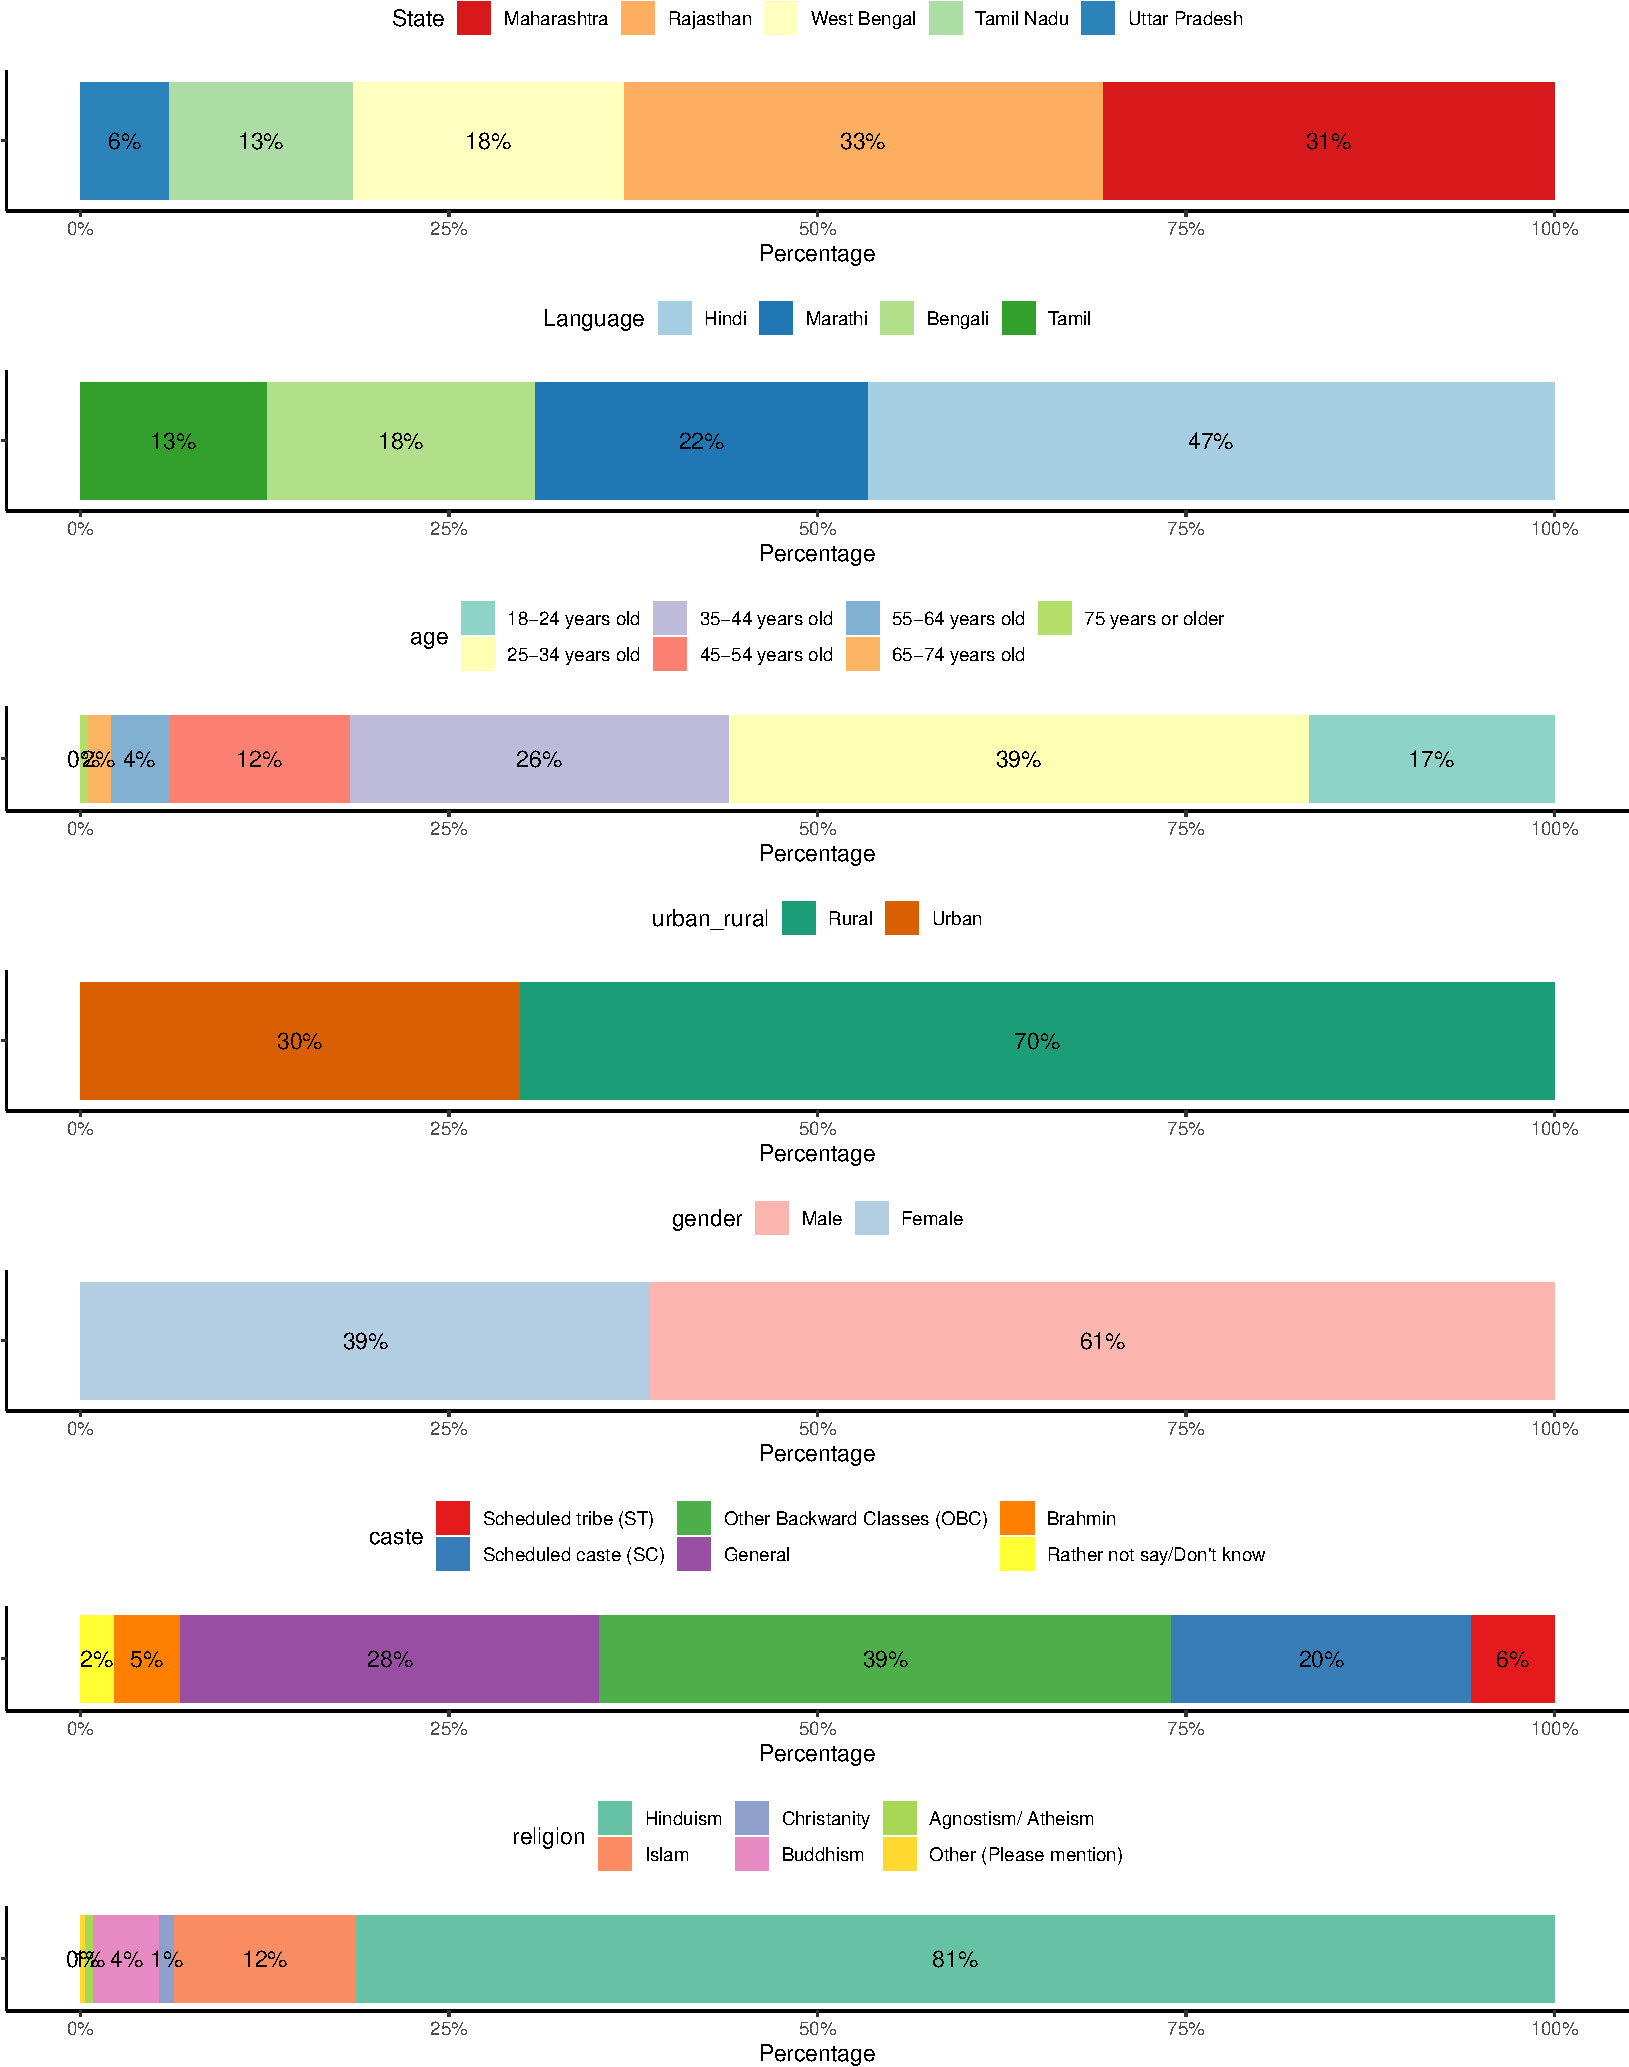
\includegraphics[width=0.8\linewidth,height=0.8\textheight]{LPGversusFirewood_files/figure-latex/unnamed-chunk-6-1}

\newpage

\hypertarget{perceived-risk-and-perceived-benefit-in-comparison}{%
\section{Perceived risk and Perceived Benefit in
comparison}\label{perceived-risk-and-perceived-benefit-in-comparison}}

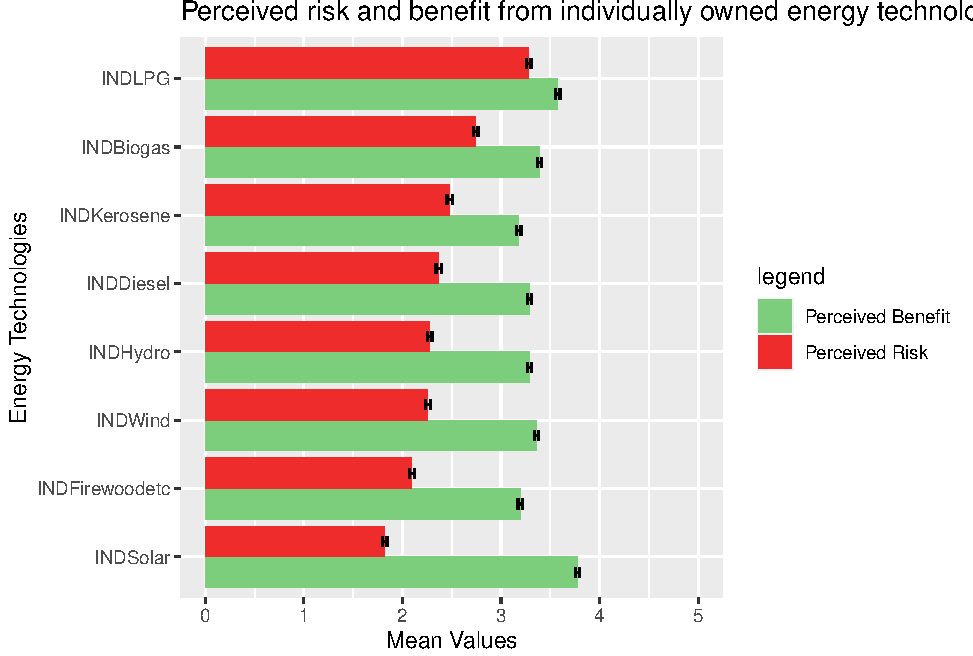
\includegraphics{LPGversusFirewood_files/figure-latex/unnamed-chunk-7-1.pdf}

\newpage

\hypertarget{t-tests}{%
\section{T-tests}\label{t-tests}}

\hypertarget{pairwise-t-test-mean-perceived-risk-and-mean-perceived-benefit-all-individually-owned-energy-technologies}{%
\subsection{Pairwise T-test: Mean perceived risk and mean perceived
benefit (all individually owned energy
technologies)}\label{pairwise-t-test-mean-perceived-risk-and-mean-perceived-benefit-all-individually-owned-energy-technologies}}

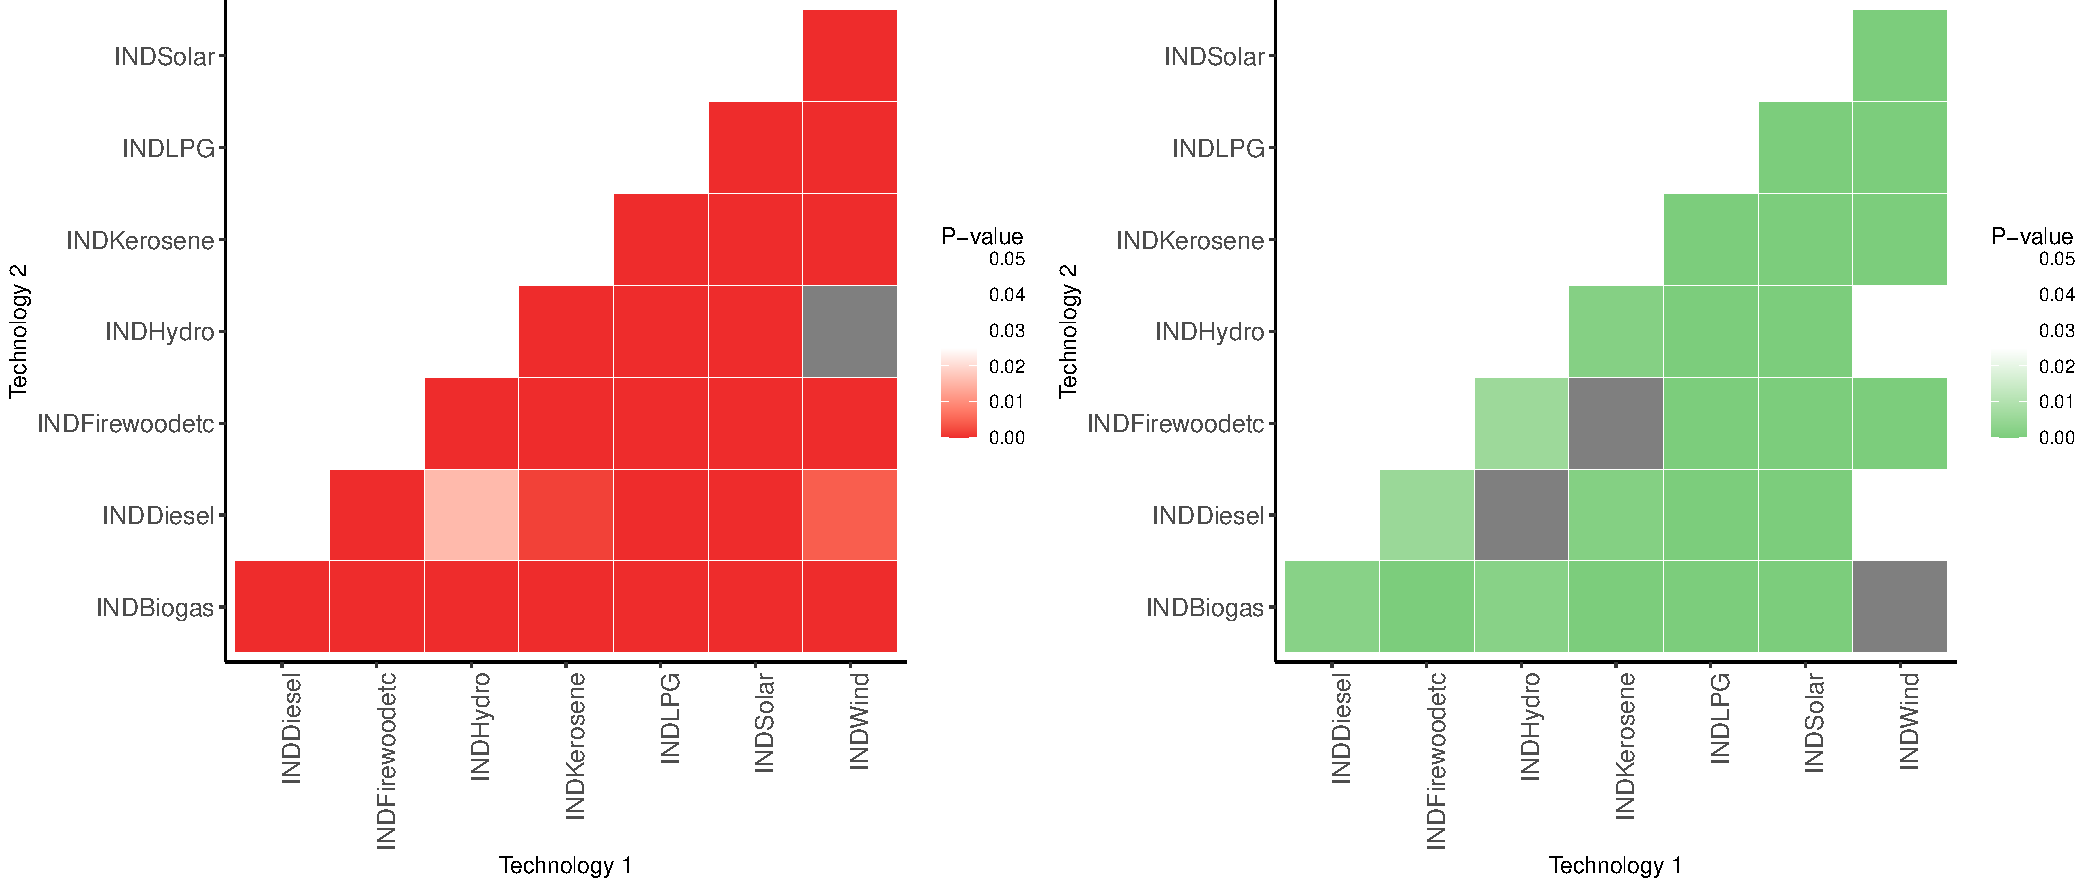
\includegraphics{LPGversusFirewood_files/figure-latex/unnamed-chunk-8-1.pdf}

\hypertarget{paired-t-test-comparing-mean-perceived-risk-and-mean-perceived-benefit-for-each-technology.}{%
\subsection{Paired T-test: Comparing mean perceived risk and mean
perceived benefit for each
technology.}\label{paired-t-test-comparing-mean-perceived-risk-and-mean-perceived-benefit-for-each-technology.}}

Null hypothesis (H0): The mean difference between perceived risk and
perceived benefit from each technology is zero. All p values are less
than 0.05 suggesting that the differences observed in the bargraph are
statistically significant.

\begin{verbatim}
## $INDBiogas
## [1] 1.726684e-68
## 
## $INDDiesel
## [1] 1.524978e-108
## 
## $INDFirewoodetc
## [1] 2.751717e-165
## 
## $INDHydro
## [1] 3.355493e-143
## 
## $INDKerosene
## [1] 1.023315e-81
## 
## $INDLPG
## [1] 2.125422e-16
## 
## $INDSolar
## [1] 0
## 
## $INDWind
## [1] 1.799622e-128
\end{verbatim}

\hypertarget{acceptance-perceived-benefit---perceived-risk}{%
\section{Acceptance = Perceived Benefit - Perceived
Risk}\label{acceptance-perceived-benefit---perceived-risk}}

Graph representing a combined acceptance scale obtained by subtracting
perceived risk from perceived benefit for each respondent

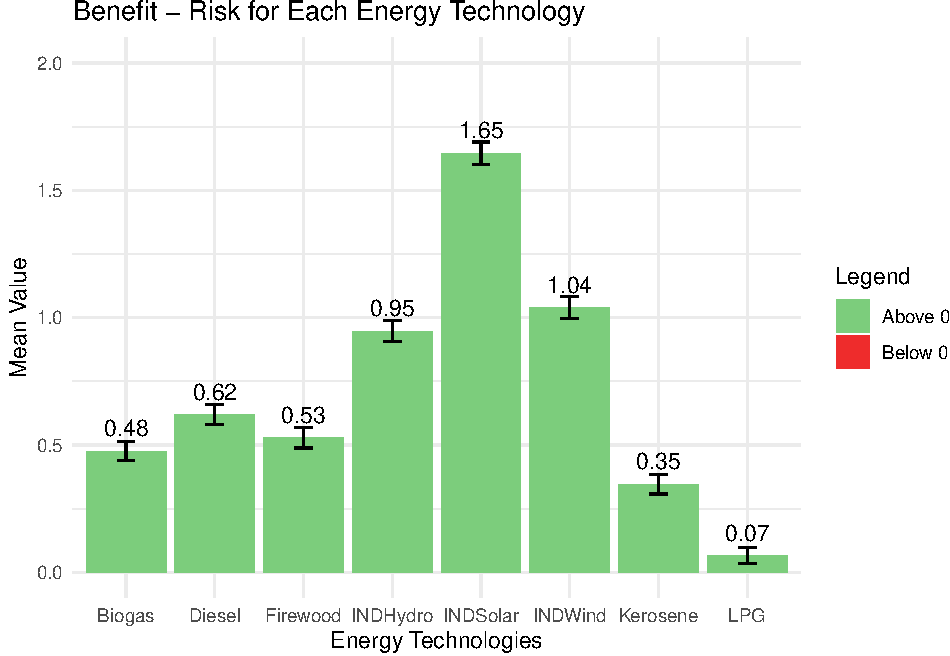
\includegraphics{LPGversusFirewood_files/figure-latex/unnamed-chunk-10-1.pdf}
\newpage

\hypertarget{linear-regression-models}{%
\section{Linear Regression Models}\label{linear-regression-models}}

\hypertarget{firewood-demographic-variables}{%
\subsection{Firewood : demographic
variables}\label{firewood-demographic-variables}}

\begingroup\setlength{\tabcolsep}{1pt}\renewcommand{\arraystretch}{0.7}

\% Table created by stargazer v.5.2.3 by Marek Hlavac, Social Policy
Institute. E-mail: marek.hlavac at gmail.com \% Date and time: Fri, Aug
18, 2023 - 12:22:51

\begin{table}[!htbp] \centering 
  \caption{Results from 2 linear regression models} 
  \label{} 
\begin{tabular}{@{\extracolsep{5pt}}lcc} 
\\[-1.8ex]\hline 
\hline \\[-1.8ex] 
 & \multicolumn{2}{c}{\textit{Dependent variable:}} \\ 
\cline{2-3} 
\\[-1.8ex] & \multicolumn{2}{c}{Risky\_INDFirewoodetc} \\ 
\\[-1.8ex] & (1) & (2)\\ 
\hline \\[-1.8ex] 
 Uppercaste & $-$0.077 & $-$0.181$^{***}$ \\ 
  & (0.050) & (0.047) \\ 
  & & \\ 
 Male & $-$0.014 & $-$0.001 \\ 
  & (0.047) & (0.044) \\ 
  & & \\ 
 Hindu & 0.011 & 0.214$^{***}$ \\ 
  & (0.058) & (0.055) \\ 
  & & \\ 
 urban\_ruralUrban & 0.534$^{***}$ & 0.146$^{***}$ \\ 
  & (0.051) & (0.056) \\ 
  & & \\ 
 age25-34 years old & $-$0.163$^{**}$ & $-$0.073 \\ 
  & (0.067) & (0.061) \\ 
  & & \\ 
 age35-44 years old & $-$0.440$^{***}$ & $-$0.228$^{***}$ \\ 
  & (0.073) & (0.069) \\ 
  & & \\ 
 age45-54 years old & $-$0.428$^{***}$ & $-$0.211$^{**}$ \\ 
  & (0.088) & (0.082) \\ 
  & & \\ 
 age55-64 years old & $-$0.406$^{***}$ & $-$0.184 \\ 
  & (0.130) & (0.121) \\ 
  & & \\ 
 age65-74 years old & $-$0.676$^{***}$ & $-$0.115 \\ 
  & (0.189) & (0.177) \\ 
  & & \\ 
 age75 years or older & 0.641$^{*}$ & 1.070$^{***}$ \\ 
  & (0.354) & (0.327) \\ 
  & & \\ 
 StateRajasthan &  & $-$0.844$^{***}$ \\ 
  &  & (0.068) \\ 
  & & \\ 
 StateTamil Nadu &  & $-$1.443$^{***}$ \\ 
  &  & (0.075) \\ 
  & & \\ 
 StateUttar Pradesh &  & $-$0.546$^{***}$ \\ 
  &  & (0.102) \\ 
  & & \\ 
 StateWest Bengal &  & $-$0.455$^{***}$ \\ 
  &  & (0.070) \\ 
  & & \\ 
 Constant & 2.207$^{***}$ & 2.631$^{***}$ \\ 
  & (0.081) & (0.080) \\ 
  & & \\ 
\hline \\[-1.8ex] 
Observations & 2,104 & 2,104 \\ 
R$^{2}$ & 0.092 & 0.235 \\ 
Adjusted R$^{2}$ & 0.088 & 0.230 \\ 
Residual Std. Error & 1.049 (df = 2093) & 0.964 (df = 2089) \\ 
F Statistic & 21.294$^{***}$ (df = 10; 2093) & 45.758$^{***}$ (df = 14; 2089) \\ 
\hline 
\hline \\[-1.8ex] 
\textit{Note:}  & \multicolumn{2}{r}{$^{*}$p$<$0.1; $^{**}$p$<$0.05; $^{***}$p$<$0.01} \\ 
\end{tabular} 
\end{table} 
\endgroup

\hypertarget{lpg-demographic-variables}{%
\subsection{LPG : demographic
variables}\label{lpg-demographic-variables}}

\begingroup\setlength{\tabcolsep}{1pt}

\renewcommand{\arraystretch}{0.7}

\% Table created by stargazer v.5.2.3 by Marek Hlavac, Social Policy
Institute. E-mail: marek.hlavac at gmail.com \% Date and time: Fri, Aug
18, 2023 - 12:22:51

\begin{table}[!htbp] \centering 
  \caption{Results from 2 linear regression models} 
  \label{} 
\begin{tabular}{@{\extracolsep{5pt}}lcc} 
\\[-1.8ex]\hline 
\hline \\[-1.8ex] 
 & \multicolumn{2}{c}{\textit{Dependent variable:}} \\ 
\cline{2-3} 
\\[-1.8ex] & \multicolumn{2}{c}{Risky\_INDLPG} \\ 
\\[-1.8ex] & (1) & (2)\\ 
\hline \\[-1.8ex] 
 Uppercaste & 0.001 & $-$0.128$^{**}$ \\ 
  & (0.054) & (0.053) \\ 
  & & \\ 
 Male & $-$0.080 & $-$0.137$^{***}$ \\ 
  & (0.051) & (0.050) \\ 
  & & \\ 
 Hindu & $-$0.119$^{*}$ & 0.027 \\ 
  & (0.063) & (0.062) \\ 
  & & \\ 
 urban\_ruralUrban & 0.086 & $-$0.011 \\ 
  & (0.056) & (0.063) \\ 
  & & \\ 
 age25-34 years old & $-$0.045 & $-$0.004 \\ 
  & (0.072) & (0.070) \\ 
  & & \\ 
 age35-44 years old & 0.079 & 0.128$^{*}$ \\ 
  & (0.078) & (0.078) \\ 
  & & \\ 
 age45-54 years old & $-$0.166$^{*}$ & $-$0.105 \\ 
  & (0.095) & (0.093) \\ 
  & & \\ 
 age55-64 years old & 0.120 & 0.128 \\ 
  & (0.139) & (0.136) \\ 
  & & \\ 
 age65-74 years old & $-$0.483$^{**}$ & $-$0.117 \\ 
  & (0.206) & (0.202) \\ 
  & & \\ 
 age75 years or older & 0.052 & 0.308 \\ 
  & (0.386) & (0.373) \\ 
  & & \\ 
 StateRajasthan &  & $-$0.226$^{***}$ \\ 
  &  & (0.077) \\ 
  & & \\ 
 StateTamil Nadu &  & $-$0.854$^{***}$ \\ 
  &  & (0.084) \\ 
  & & \\ 
 StateUttar Pradesh &  & $-$0.023 \\ 
  &  & (0.117) \\ 
  & & \\ 
 StateWest Bengal &  & 0.250$^{***}$ \\ 
  &  & (0.080) \\ 
  & & \\ 
 Constant & 3.418$^{***}$ & 3.516$^{***}$ \\ 
  & (0.088) & (0.092) \\ 
  & & \\ 
\hline \\[-1.8ex] 
Observations & 2,139 & 2,139 \\ 
R$^{2}$ & 0.012 & 0.086 \\ 
Adjusted R$^{2}$ & 0.007 & 0.080 \\ 
Residual Std. Error & 1.144 (df = 2128) & 1.101 (df = 2124) \\ 
F Statistic & 2.545$^{***}$ (df = 10; 2128) & 14.342$^{***}$ (df = 14; 2124) \\ 
\hline 
\hline \\[-1.8ex] 
\textit{Note:}  & \multicolumn{2}{r}{$^{*}$p$<$0.1; $^{**}$p$<$0.05; $^{***}$p$<$0.01} \\ 
\end{tabular} 
\end{table} 
\endgroup

Table 1 and 2 :

\begin{enumerate}
\def\labelenumi{\arabic{enumi}.}
\tightlist
\item
  Uppercaste, Male, Hindu and urban\_rural are binary variables.
\item
  Reference for age variables is 18-24 years old
\item
  Reference for State is Maharashtra
\end{enumerate}

\hypertarget{linear-regression-model---stove-ownership-by-four-groups---ilpg-iitraditonal-stoveincluding-firewood-iiiboth-and-ivother}{%
\section{Linear Regression model - stove ownership by four groups -
(i)LPG, (ii)Traditonal Stove(Including Firewood), (iii)Both and
(iv)Other}\label{linear-regression-model---stove-ownership-by-four-groups---ilpg-iitraditonal-stoveincluding-firewood-iiiboth-and-ivother}}

\begingroup\setlength{\tabcolsep}{1pt}

\renewcommand{\arraystretch}{0.7}

\% Table created by stargazer v.5.2.3 by Marek Hlavac, Social Policy
Institute. E-mail: marek.hlavac at gmail.com \% Date and time: Fri, Aug
18, 2023 - 12:22:51

\begin{table}[!htbp] \centering 
  \caption{Results from 2 linear regression models} 
  \label{} 
\begin{tabular}{@{\extracolsep{5pt}}lcc} 
\\[-1.8ex]\hline 
\hline \\[-1.8ex] 
 & \multicolumn{2}{c}{\textit{Dependent variable:}} \\ 
\cline{2-3} 
\\[-1.8ex] & Risky\_INDLPG & Risky\_INDFirewoodetc \\ 
\\[-1.8ex] & (1) & (2)\\ 
\hline \\[-1.8ex] 
 urban\_ruralUrban & 0.074 & 0.397$^{***}$ \\ 
  & (0.091) & (0.083) \\ 
  & & \\ 
 Hindu & $-$0.086 & 0.159$^{*}$ \\ 
  & (0.089) & (0.081) \\ 
  & & \\ 
 Male & 0.099 & $-$0.020 \\ 
  & (0.070) & (0.064) \\ 
  & & \\ 
 Uppercaste & $-$0.049 & $-$0.157$^{**}$ \\ 
  & (0.076) & (0.069) \\ 
  & & \\ 
 age25-34 years old & $-$0.069 & $-$0.025 \\ 
  & (0.102) & (0.093) \\ 
  & & \\ 
 age35-44 years old & 0.018 & $-$0.234$^{**}$ \\ 
  & (0.116) & (0.106) \\ 
  & & \\ 
 age45-54 years old & $-$0.186 & $-$0.106 \\ 
  & (0.135) & (0.123) \\ 
  & & \\ 
 age55-64 years old & 0.245 & 0.031 \\ 
  & (0.185) & (0.169) \\ 
  & & \\ 
 age65-74 years old & 0.138 & 0.116 \\ 
  & (0.317) & (0.289) \\ 
  & & \\ 
 age75 years or older & 0.805 & 1.523$^{**}$ \\ 
  & (0.657) & (0.598) \\ 
  & & \\ 
 groupTraditional & 0.083 & $-$0.498$^{***}$ \\ 
  & (0.168) & (0.154) \\ 
  & & \\ 
 groupBoth & $-$0.009 & $-$0.319$^{***}$ \\ 
  & (0.095) & (0.087) \\ 
  & & \\ 
 groupOther & $-$0.952$^{***}$ & $-$1.110$^{***}$ \\ 
  & (0.156) & (0.142) \\ 
  & & \\ 
 Constant & 3.451$^{***}$ & 2.211$^{***}$ \\ 
  & (0.129) & (0.118) \\ 
  & & \\ 
\hline \\[-1.8ex] 
Observations & 1,034 & 1,034 \\ 
R$^{2}$ & 0.057 & 0.150 \\ 
Adjusted R$^{2}$ & 0.045 & 0.140 \\ 
Residual Std. Error (df = 1020) & 1.110 & 1.011 \\ 
F Statistic (df = 13; 1020) & 4.710$^{***}$ & 13.895$^{***}$ \\ 
\hline 
\hline \\[-1.8ex] 
\textit{Note:}  & \multicolumn{2}{r}{$^{*}$p$<$0.1; $^{**}$p$<$0.05; $^{***}$p$<$0.01} \\ 
\end{tabular} 
\end{table} 
\endgroup

\end{document}
